\documentclass[a4paper,12pt, twoside]{article}
\usepackage[a4paper, left=2.5cm, right=2.5cm, top=2.5cm, bottom=2.5cm, bindingoffset=0.5cm]{geometry}
\usepackage[utf8x]{inputenc}
\usepackage{polski}
\usepackage[polish]{babel}
\usepackage{graphicx}
\usepackage{indentfirst}
\usepackage{float}
\usepackage{caption}
\usepackage{adjustbox}
\usepackage{array}
\usepackage{makecell}
\usepackage{amsmath}
\usepackage{enumitem}
\usepackage{afterpage}
\usepackage{subfig}
\usepackage{hyperref}
\usepackage{url}
\renewcommand\thesection{\arabic{section}.}
\renewcommand\thesubsection{\arabic{section}.\arabic{subsection}.}
\renewcommand\thesubsubsection{\arabic{section}.\arabic{subsection}.\arabic{subsubsection}.}
\frenchspacing
\setlength{\parindent}{.5cm}
\makeatletter
\setlength{\@fptop}{0pt}
\makeatother
\linespread{1.5}
\begin{document}
	\newpage
	\thispagestyle{empty}
	\begin{center}
		
		\begin{figure}
			\centering
			
\includegraphics[width=7cm]{images/polsl_logo.jpg}
			\vspace{.5cm}
		\end{figure}
		
		{\fontsize{17}{17}\selectfont
			\textsc{Politechnika Śląska \\[.3cm]
				Wydział Automatyki, Elektroniki i Informatyki  \\[.3cm]
				Kierunek Automatyka i Robotyka  \\[1.5cm]}
			\textbf{Projekt inżynierski \\[0.7cm]}}
		
		\Large
		{Elektroniczna plakietka konfigurowana z urządzenia mobilnego \\[3.5cm]}
		\Large{\begin{flushleft}
				Autor: Jakub Legutko\\
				Kierujący pracą: dr inż. Grzegorz Dziwoki\\[0.3cm]
		\end{flushleft}}
		
		\normalsize
		\vfill Gliwice, styczeń 2019
	\end{center}
	\newpage
	\newpage
	\thispagestyle{empty}
	\tableofcontents
	\newpage
	%\leavevmode\thispagestyle{empty}\newpage
	\newpage
	\clearpage
	\setcounter{page}{1}
	
	\section{Wstęp}
	
	\subsection{Wprowadzenie}
	Zmiany klimatyczne są coraz bardziej widoczne na świecie. Wycinka drzew jest jednym z głównych powodów wzrostu emisji gazów cieplarnianych\cite{clima_causes}, ograniczenie jej wpłynie pozytywnie na poziom ${CO_{2}}$ w atmosferze, co przełoży się na polepszenie klimatu. 
	
	Druk wizytówek oraz identyfikatorów pochłania znaczące ilości papieru, oraz tuszu w skali globalnej ze względu na ich jednorazowe wykorzystanie w większości przypadków. Z tego powodu ważne jest znalezienie alternatywnej metody. Gdyby zamiast papieru wykorzystać urządzenie, z którego można korzystać wielokrotnie poprzez zmianę wyświetlanych danych, zmniejszylibyśmy zapotrzebowanie na papier, zmniejszając jednocześnie emisję dwutlenku węgla. Oprócz papieru potrzebnego do wytworzenia plakietek nie będziemy również marnować toneru, którego produkcja pochłania około 3.2 kilograma gazów cieplarnianych\cite{cartidge_production} na kartridż zawierający 200 gramów toneru. Kolejną rzeczą jest recykling, któremu trzeba poddać niepotrzebne już identyfikatory oraz zużyte do produkcji ich kartridże.
	
	Idealnym rozwiązaniem takiego problemu wydaje się papier elektroniczny (ang. \textit{e-paper}). Wyświetlane na nim dane można modyfikować dowolną ilość razy, dzięki czemu może być wykorzystywany wielokrotnie, nie powodując zużycia dodatkowych surowców. Po wyświetleniu dostarczonych danych nie jest już zużywana energia. Przez co może być używany bez dodatkowych baterii lub innego dodatkowego źródła zasilania.
	\newpage
	
	
	\subsection{Cel projektu}
	Celem projektu inżynierskiego jest zaprojektowanie elektronicznej plakietki identyfikującej mogącej zastąpić identyfikatory lub wizytówki z wykorzystaniem wyświetlacza typu e-papier. Prezentowane dane są przygotowywane i przesyłane przy pomocy urządzenia mobilnego za pomocą napisanej aplikacji.

	\subsection{Założenia projektowe}
	\begin{itemize}
		\item użycie wyświetlacza wykonanego w technologii papieru elektronicznego
		\item mobilność działania plakietki 
		\item łączność bezprzewodowa pomiędzy ekranem a urządzeniem wysyłającym dane
		\item aplikacja na system Android
		\item przechowywanie w aplikacji wpisów z danymi do wyświetlania
		\item wyświetlanie danych w różnych miejscach na ekranie 
		\item przechowywanie układów wyświetlania danych w pamięci urządzenia
	\end{itemize}
	\newpage
	
	\subsection{Opis projektu}
	Do realizacji projektu wykonano prototyp urządzenia składający się z mikrokontrolera oraz ekranu w technologii papieru elektronicznego. Dla urządzenia wysyłającego dane wykonano aplikację mobilną, posiadającą funkcję wysyłania oraz przechowywania danych. 
	
	Wybór jednostki sterującej wybrano głównie dla prostoty wykonania prototypu. Zdecydowano się na mikrokontroler zawierający zintegrowaną technologie do połączeń bezprzewodowych tj. \textit{Bluetooth}\cite{bluetooth} lub \textit{Wi-Fi}\cite{wifi}. 
	
	Ostatecznie zdecydowano o wykorzystaniu protokołu \textit{Bluetooth} do bezprzewodowej transmisji danych z urządzenia mobilnego do mikrokontrolera. Głównym powodem dla wyboru \textit{Bluetootha} jest występowanie tej technologii w zdecydowanej większości urządzeń mobilnych dostępnych na rynku, dzięki czemu wykonany projekt będzie mógł być wykorzystany przez szeroki zakres urządzeń.
	
	\begin{flushleft}
	Wykonanie projektu przebiegło w kilku etapach:
	\begin{itemize}
	    \item wykonanie prototypu urządzenia
	    \item napisanie programu sterującego mikrokontrolerem
	    \item napisanie aplikacji dla urządzenia mobilnego
	    \item przeprowadzenie testów urządzeń i aplikacji
	\end{itemize}
	\end{flushleft}
	\newpage
	\section{Realizacja projektu}
	Do wykonania projektu użyto następujących technologii oraz narzędzi.
	
	\subsection{Narzędzia programistyczne}
	\subsubsection{Android Studio}
	Android Studio jest oficjalnym zintegrowanym środowiskiem programistycznym \textit{z ang. integrated development environment}\cite{ide} do produkcji aplikacji na system Android, bazowanym na IntelliJ IDEA.
	
	\begin{figure}[H]
			\vspace{.5cm}
			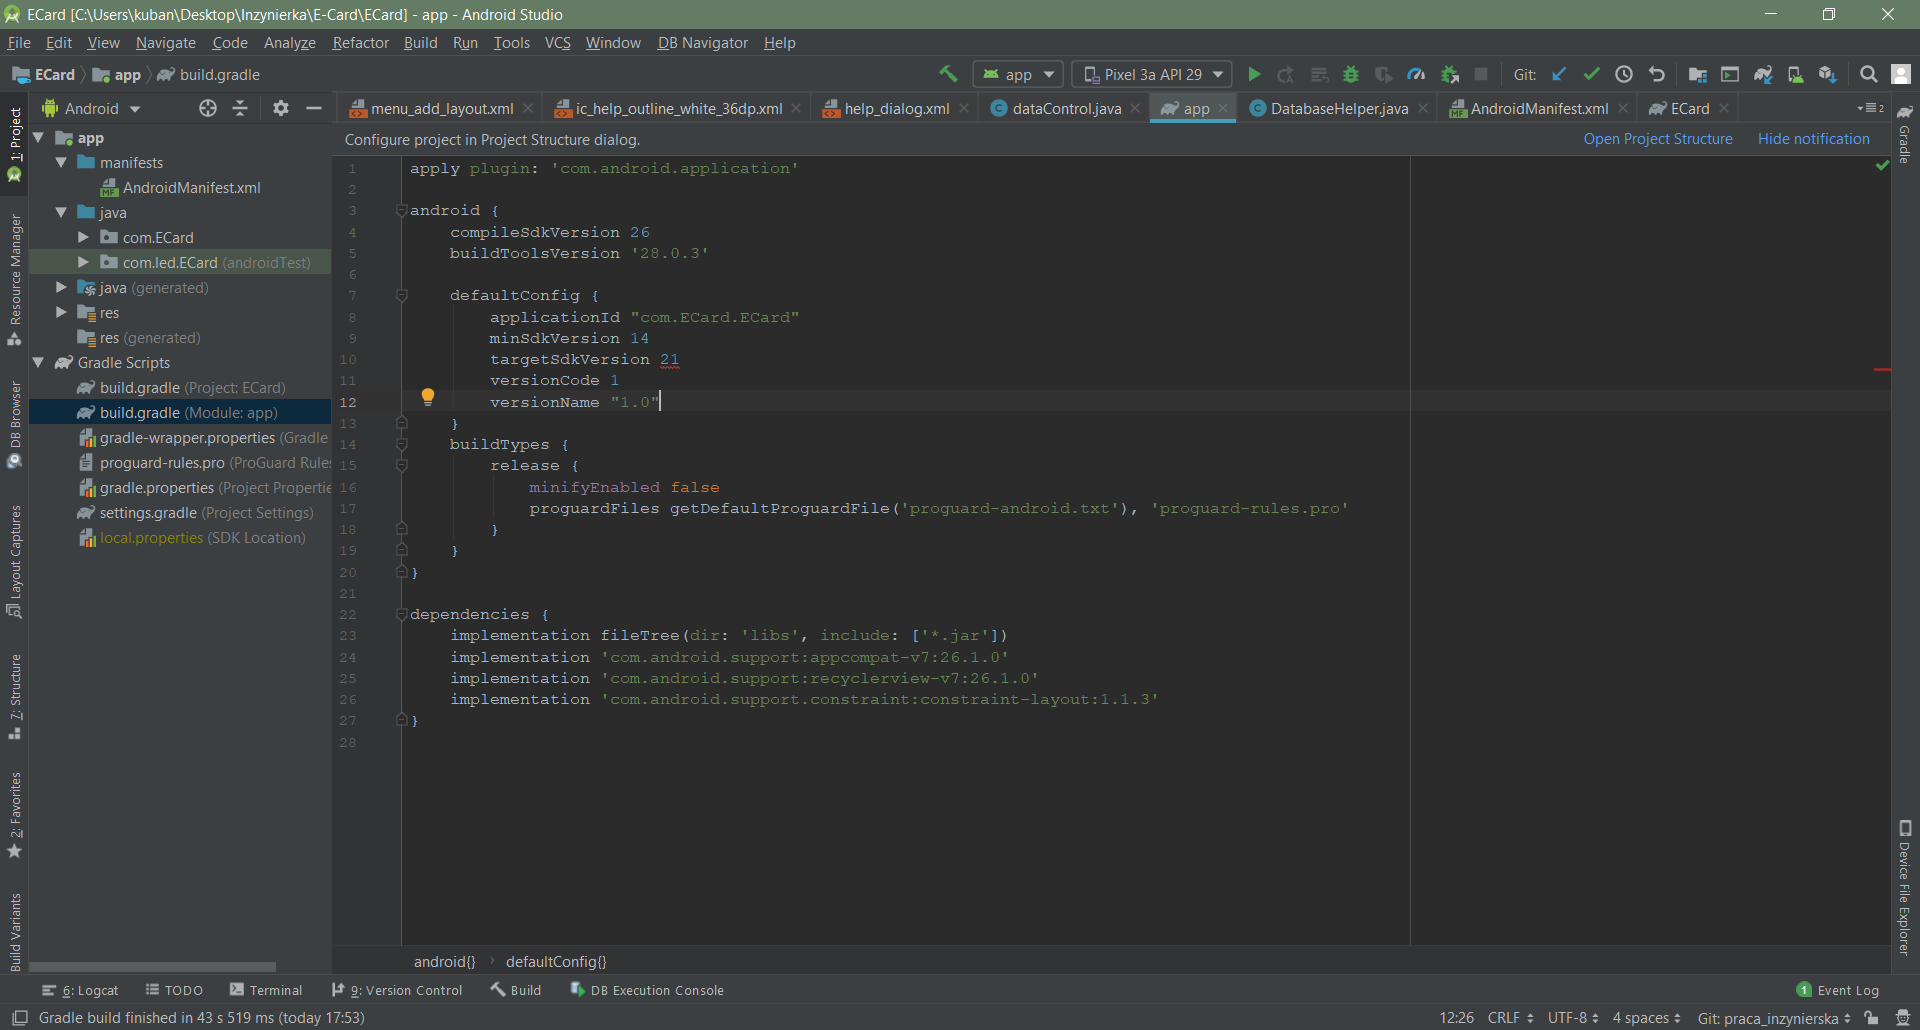
\includegraphics[width=16cm]{images/rys4_android.png}
			\vspace{.5cm}
			\caption{Widok Android Studio}
            \label{fig:androidstudio}
	\end{figure}
	
	\newpage
	\begin{flushleft}
	Oprócz posiadanie czołowych możliwości edycji kodu i wbudowanych zaawansowanych narzędzi programistycznych cechuje się również:
	\begin{itemize}
	    \item elastycznym narzędziem służącym do budowania projektów opartym na Gradle\cite{gradle}
	    \item szybkim i bogatym w funkcje emulatorem
	    \item zunifikowanym środowiskiem do produkcji aplikacji na wszystkie urządzenia z systemem android
	    \item szablonami kodu i integracją z GitHub
	    \item obszernymi narzędziami do testowania kodu i aplikacji
	    \item narzędziami do wykrywania błędów składni \textit{Lint}\cite{lint}, niezgodności wersji i innych błędów
	    \item wsparciem \textit{Native Development Kit}\cite{ndk}
	\end{itemize}
	\end{flushleft}
	\newpage
	\subsubsection{Git}
	\vspace{.5cm}
	Git jest to rozproszony system kontroli wersji stworzony przez Linusa Torvaldsa. Jest to wolne oprogramowanie opublikowane na licencji GNU GPL v2.0.
	
	Git śledzi wszelkie różnice dokonane w plikach, pozwala wrócić do dowolnej wcześniejszej wersji. Daje możliwość podglądu wszystkich zmian, które były wykonane w pliku z dokładnością to zmian w każdej linii kodu. Jest zbudowany do pracy w wiele osób, widzimy zmiany wprowadzone przez innych.
	
	Jedną z najbardziej przydatnych funkcji są gałęzie. Dzięki nim wiele osób może pracować nad różnymi funkcjonalnościami aplikacji bez przeszkadzania sobie, a następnie w prosty i szybki sposób zmiany te można dołożyć do głównej gałęzi projektu.
		\begin{figure}[H]
			\centering
			\vspace{.5cm}
			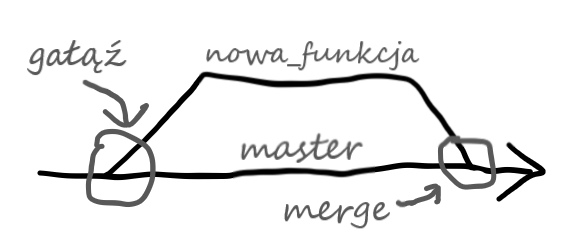
\includegraphics[width=11cm]{images/rys1_branches.png}
			\vspace{.5cm}
			\caption{Schemat wykorzystania gałęzi}
            \label{fig:branching}
		\end{figure}

	Uzyskujemy dzięki temu kontrole nad projektem, która przekłada się na mniejszą ilość błędów większą ilość czasu, którą można przeznaczyć na tworzenie nowych funkcjonalności niż na ręczne składanie kodu wielu osób.\cite{git}
	
	\newpage
	\subsubsection{GitKraken}
	\vspace{.5cm}
	GitKraken jest graficznym klientem Gita dla wielu platform zbudowanym przez AxoSoft w 2014 roku. GitKraken uproszcza skomplikowane komendy tekstowe wiersza poleceń\cite{cli} wykorzystywanego do obsługi GIT. Pozwala na korzystanie ze zdalnych repozytoriów poprzez integrację z takimi systemami jak np. GitHub, GitLab czy Bitbucket. W aplikacji wbudowane są narzędzia rozwiązywania konfliktów scalania, dostępny jest również edytor tekstowy. 
	\begin{figure}[H]
			\vspace{1cm}
			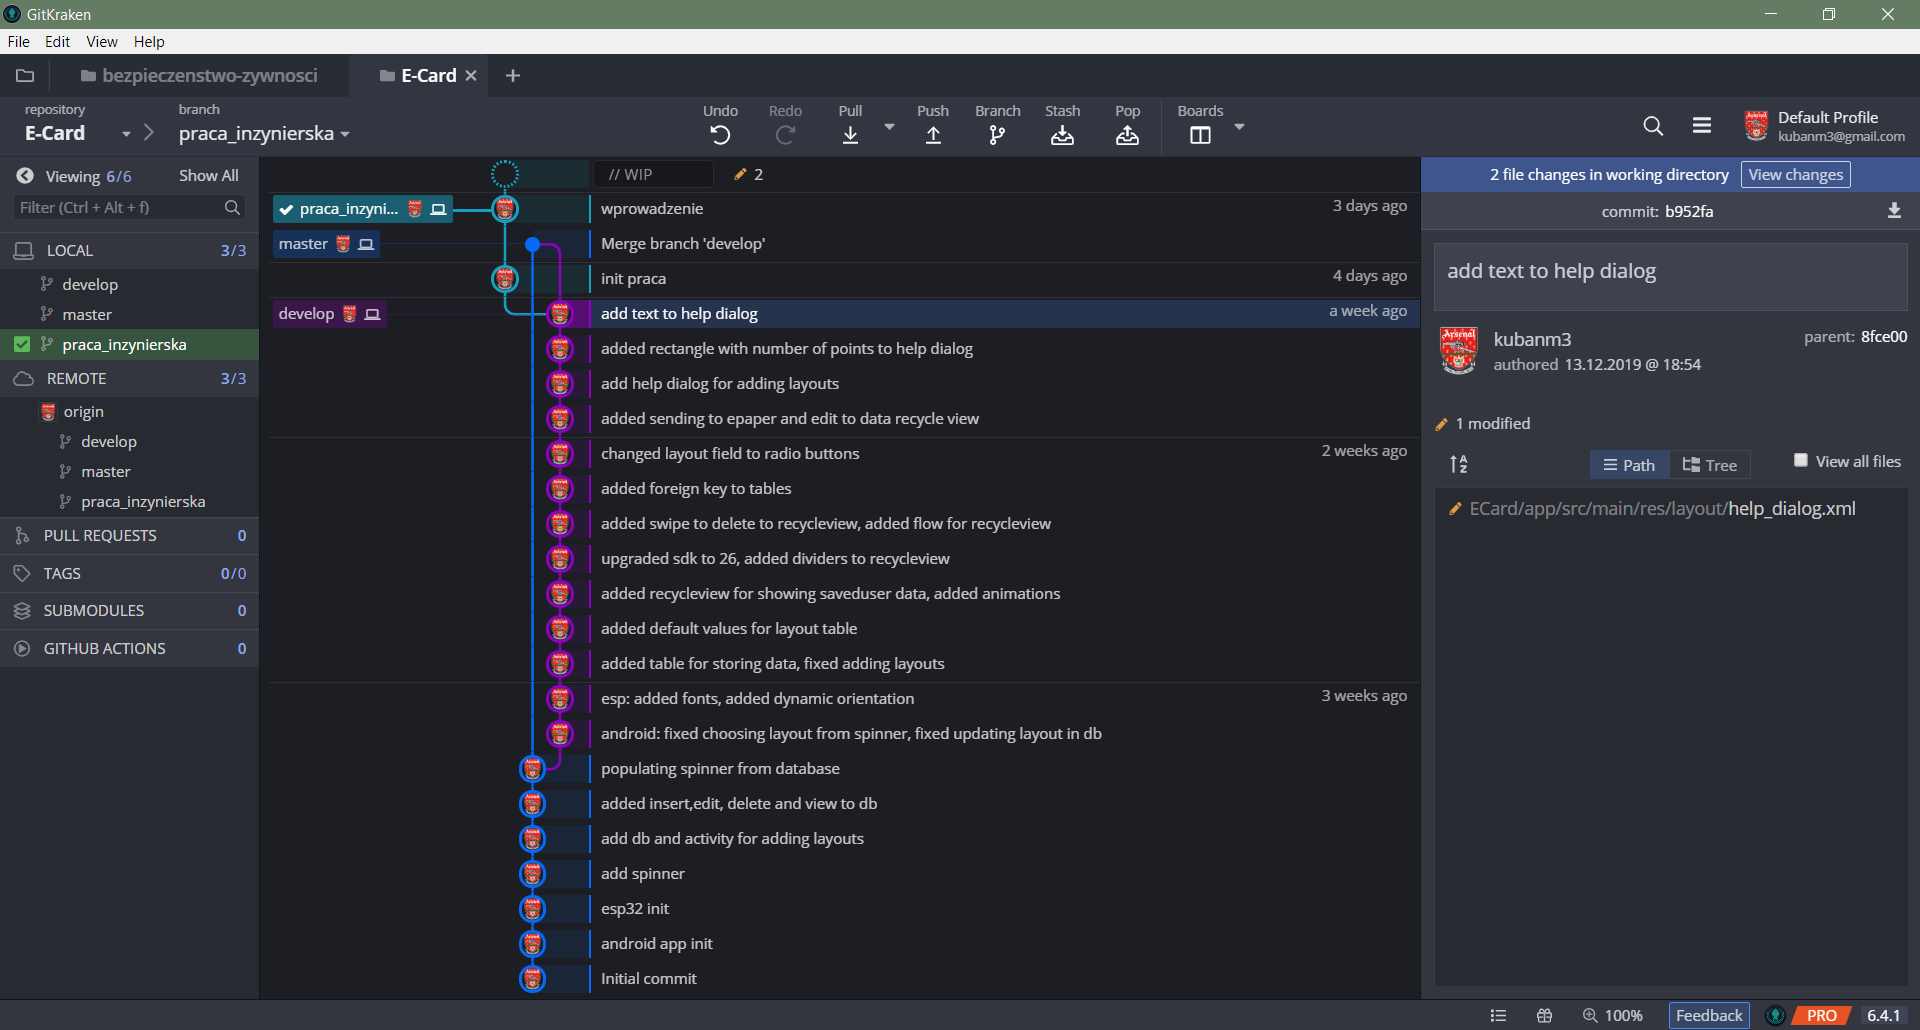
\includegraphics[width=16cm]{images/rys2_gitkraken.png}
			\vspace{.5cm}
			\caption{Repozytorium przedstawione w GitKraken}
            \label{fig:gitkraken}
	\end{figure}
		
	\vspace{.5cm}
	W projektach, gdzie pracuje jednocześnie wiele osób graficzna wizualizacja ułatwia kontrole nad wieloma gałęziami i zapanowanie nad projektem.   
	
	\newpage
	\subsubsection{Arduino IDE}
	Arduino IDE jest wieloplatformowym zintegrowanym środowiskiem deweloperskim napisanym w języku C oraz C++. Oparty jest na wolnej licencji GNU GPL v2.0. Używane jest do pisania oraz wgrywania programów do kompatybilnych płytek Arduino. Możliwe jest również wykorzystanie go do wgrywania na płytki firm trzecich za pomocą dołączonych do nich sterowników. 
	
	Programy pisane są w językach C oraz C++ używając specjalnych struktur kodowania. Udostępnionych jest na nie wiele bibliotek obsługujących szeroką gamę czujników, serw czy wyświetlaczy.
	
	\begin{figure}[H]
			\vspace{.5cm}
			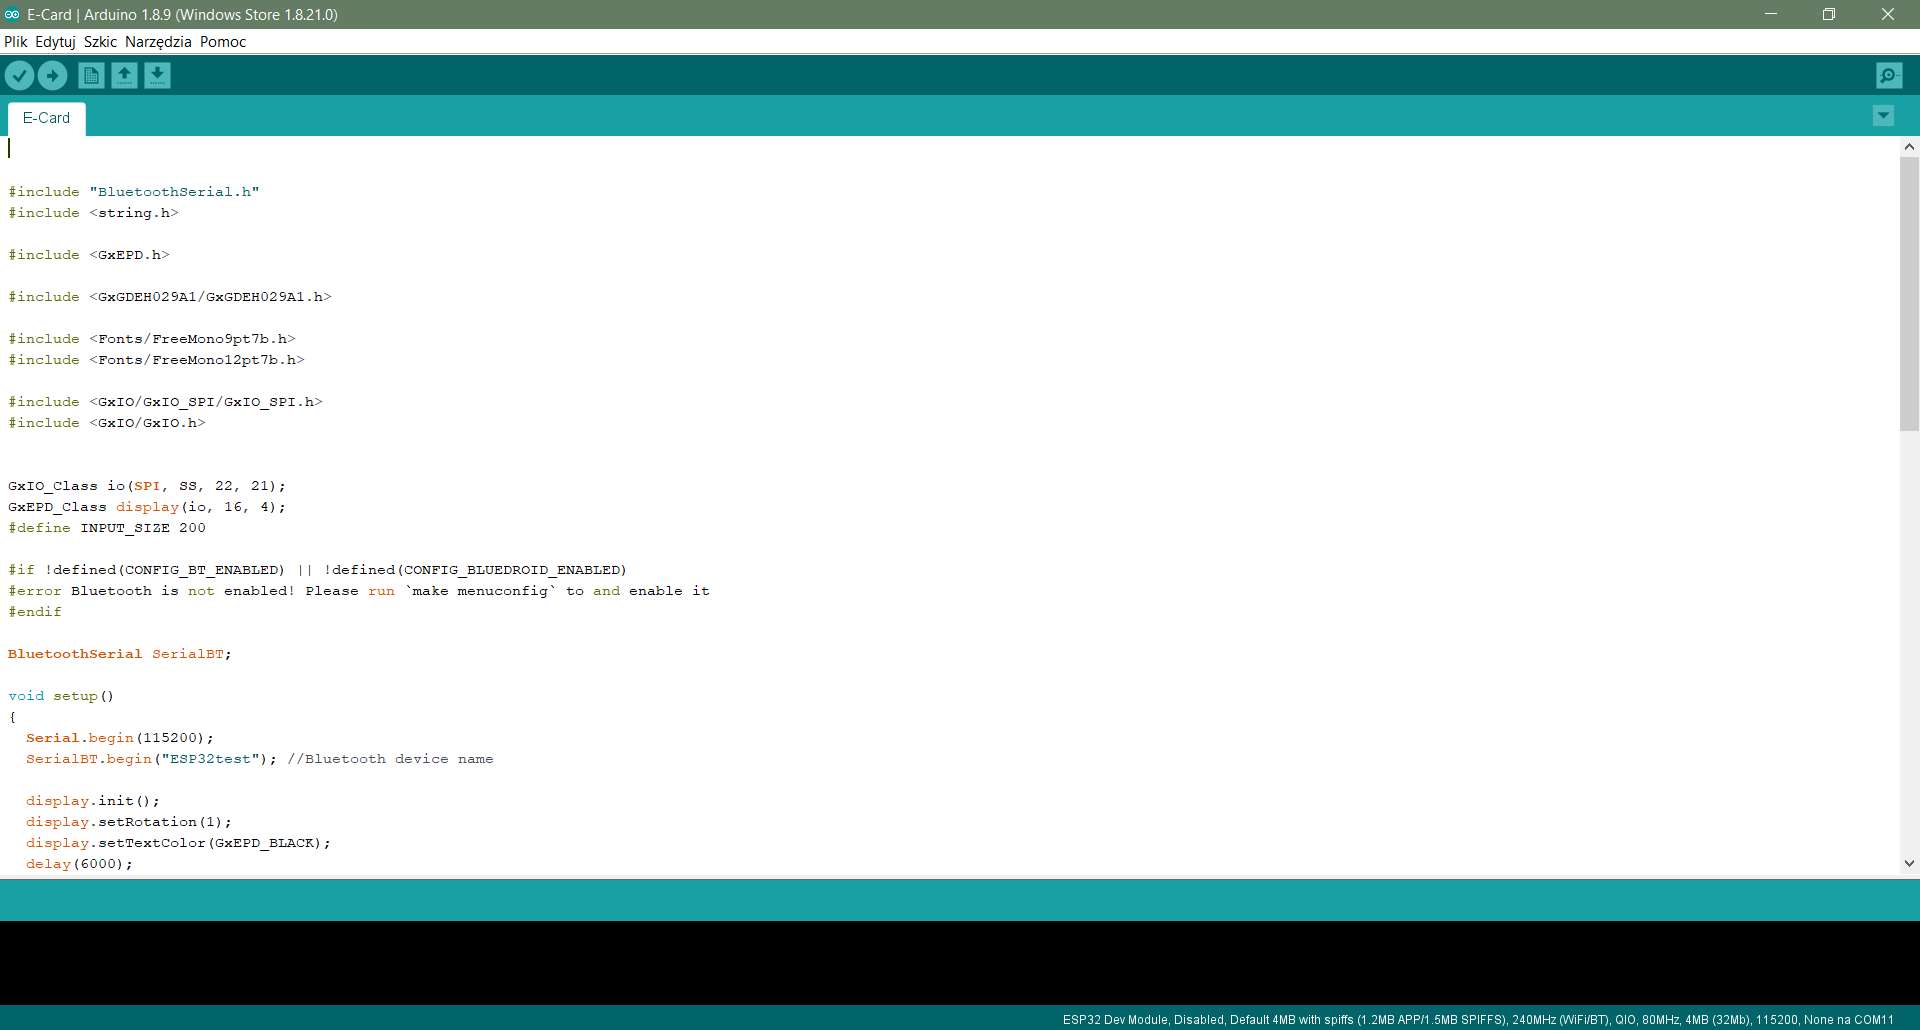
\includegraphics[width=16cm]{images/rys3_arduino.png}
			\vspace{.5cm}
			\caption{Widok Arduino IDE}
			\vspace{1cm}
            \label{fig:arduinoide}
	\end{figure}

	Napisany przez użytkownika kod do działania potrzebuje tylko dwie podstawowe funkcje. Są nimi setup() do rozpoczęcia działania i ustawienia początkowych parametrów oraz loop(), która jest pętlą główną programu.
	
	\newpage
	Środowisko zawiera trzy najważniejsze podprogramy, którymi są:
	\begin{itemize}
	\item Edytor kodu źródłowego - piszemy w nim nasz program. Zawiera takie funkcje jak sprawdzanie składni czy auto-formatowanie kodu.
	\item Kompilator - wykonuje konwersje kodu wykonywalnego w plik tekstowy z szesnastkowym kodowaniem zrozumiałym przez mikrokontroler.
	\item Loader - przesyła odpowiedni plik do Arduino.
	\end{itemize}
	
	\newpage
	\subsection{Wykorzystane technologie}
	\subsubsection{Java}
	Java jest opartym na klasach obiektowym językiem programowania. W programowaniu dla Androida wykorzystuje się przygotowane dla niego SDK\textit{ z ang. Software development kit}\cite{sdk}.
	
	W systemie Android cykl życia aplikacji wygląda inaczej niż w aplikacjach kontrolowanych przez \textit{Java Virtual Machine}\cite{jvm}. Nie występuje tutaj klasyczna metoda jaką jest \textit{public static main(String[] args) {...}} a mamy za to nowe metody w klasie aktywności jakimi są onCreate, onPause, onDestroy, onRestart i inne. Metody te wykorzystywane są w różnych momentach działania aktywności co możemy zobaczyć na rysunku \ref{fig:lifecycle}.

	
	\begin{figure}[H]
	        \centering
			\vspace{.5cm}
			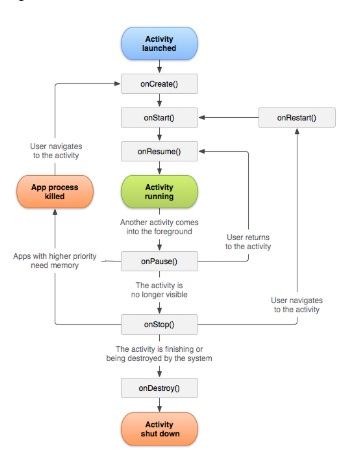
\includegraphics[width=10cm]{images/rys6_androidlifecycle.png}
			\vspace{.5cm}
			\caption{Uproszczony ilustracja cyklu życia aktywności\cite{lifecycle}}
            \label{fig:lifecycle}
	\end{figure}
	
	Metoda onCreate jest metodą uruchamianą jako pierwszą. Tutaj ustawiamy widok aktywności. W niej także przypisujemy elementy do kodu, który chcemy aby się wykonywał po interakcji z określoną kontrolką.
		
	Widoki aplikacji są budowane w wielu różnych plikach XML oraz w klasach activity, gdzie można również tworzyć elementy programowo.
	
	W przeciwieństwie do \textit{JVM} gdzie mamy pełną kontrolę nad cyklem życia procesu. W Androidzie aktywności są ciągle aktywne w tle po zamknięciu aplikacji przez użytkownika. To system steruje, kiedy aktywności zostają całkowicie wyłączone i usunięte z pamięci urządzenia. 
	
	Po zamknięciu aplikacji mogą one ciągle działać w tle jedynie zmniejszając część używanej przez siebie pamięci oraz zamknięciu niektórych z używanych procesów jak na przykład połączenie Bluetooth, GPS czy łączność z internetem. Takie rozwiązanie ma sprzyjać szybkości i zużyciu zasobów podczas ponownego uruchamiania aplikacji przez co polepszać wykorzystanie baterii\cite{batterysave}.
	
	Więcej informacji oraz większa liczba szczegółów można zaczerpnąć z książki \textit{Android Programming: The Big Nerd Ranch Guide (3rd Edition)}\cite{androidprogramming}.
	
	\vspace{1cm}
	\subsubsection{SQLite}
	SQLite jest relacyjną bazą danych dostępną na licencji \textit{public domain}\cite{publicdomain} zbudowaną w 2000 roku przez Richarda Hippa. SQLite implementuje mały rozmiarem (mniej niż 600KiB), szybki, samodzielny  silnik SQL \textit{(ang. Structured Query Language)}. Jest najczęściej używanym silnikiem baz danych na świecie. Występuje we wszystkich telefonach mobilnych oraz większości komputerów.Do działania nie potrzebuje dodatkowego procesu serwera, zapisuje i odczytuje dane bezpośrednio ze zwykłych dysków danych. Format plików jest uniwersalny, możliwe jest używanie jej i kopiowanie baz po stworzeniu pomiędzy systemami 32 lub 64 bitowymi czy wykorzystującymi architektury kolejności bajtów \textit{big-endian} lub \textit{little-endian}\cite{endian}. SQLite jest starannie testowana przed wypuszczenie każdej nowej wersji oprogramowania. Automatyczne testy osiągają 100 procent pokrycia rozgałęzień\cite{branchcoverage}. Na co dzień SQLite jest wspierany przez międzynarodowy zespół programistów pracujących nad nim w pełnym wymiarze czasu. Kod źródłowy jest otwarty i dostępny dla każdego\cite{sqlite}.
	
	Szczegółowe informacje dotyczące SQLite i jej zasad działania i użytych technologii na najniższym poziomie dostępne są w książce \textit{SQLite Forensics (2018)}\cite{sqliteforensics}. 
	
	\vspace{1cm}
	\subsubsection{Arduino code}
	Kod Arduino pisany jest w C++ z dołączonymi do niego specjalnymi metodami i funkcjami wykorzystywanymi i napisanymi specjalnie dla płytek Arduino i ich klonów. Ze względu na otwartą naturę projektu Arduino, biblioteki i inne zasoby posiadają obszerną liczbę pozycji. Arduino posiada wiele wbudowanych bibliotek dostarczających podstawowe funkcjonalności większości elementów, które można podłączyć do płytki. 
	
	\begin{flushleft}
	\vspace{.5cm}Programowanie programów dla Arduino jest podzielone na dwie główne części:
	\begin{enumerate}
	    \item  
	    \textbf{setup()}, ustalamy tutaj początkowy stan Arduino po uruchomieniu. Wykonywany jest tylko jeden raz.	
	    \begin{itemize}
	        \item ustalamy początkowy stan pinów
	        \item przypisujemy zmienne
	        \item tworzymy klasy
    	\end{itemize}
    	\item  
	    \textbf{loop()}, uruchamiana jest po skończeniu działania setup(). Uruchamiana jest w nieskończonej pętli. Opisana jest w niej główna logika programu.
	\end{enumerate}
	
	\flushleft\vspace{.5cm}Podstawowy zarys jak programować w Arduino można opisać w czterech krokach.\cite{stepsarduino} 
	
	
	\begin{enumerate}
	    \item \textbf{Konfiguracja} - najczęściej będzie opisana w \textit{setup()}. Wykonywana tylko raz do opisu pinów, przypisania zmiennych, kalibracji czujników.
	    \item \textbf{Dane wejściowe} - po rozpoczęciu \textit{loop()} powinniśmy przypisać przychodzące dane do zmiennych do dalszego wykorzystania lub do wywołania odpowiednich kawałków kodu zależnie od przychodzących danych, tj. jako instrukcje warunkowe.  
	    \item \textbf{Obsługa danych} - konwersja danych w łatwiejsze do obsługi przez programistę np. przypisanie danych z portu szeregowego do tablic po zastosowaniu odpowiednich kodowań. Przystosowanie danych do dalszego przesłania jeżeli wymaga tego program.
	    \item \textbf{Dane wyjściowe} - np. wysyłanie przygotowanych danych w odpowiedniej formie na port szeregowy do dalszej obróbki przez inne systemy czy przełączanie pinów na stany odpowiadające logice kodu.
	\end{enumerate}
	\end{flushleft}
	
	\vspace{1cm}
    Biblioteki wykorzystywane w programy Arduino składają się z plików źródłowych z rozszerzeniem \textit{.cpp}, oraz plików nagłówkowych \textit{.h}. Pliki nagłówkowe opisują strukturę biblioteki. Są w niej również deklarowane wszystkie zmienne i funkcje wykorzystywane przez bibliotekę. W plikach źródłowych \textit{.cpp} zawarte są implementowane kody funkcji.
    
	\section{Opis i specyfikacja urządzenia}
	Elektroniczna plakietka konfigurowana z urządzenia mobilnego składa się z dwóch fizycznych części. Urządzenia mobilnego z zainstalowanym oprogramowaniem napisanym do obsługi tego projektu oraz urządzenie będące fizyczną częścią projektu składające się z mikrokontrolera oraz wyświetlacza w technologii elektronicznego papieru.

    Przedstawię w tym rozdziale ogólny schemat projektu, wybrane podzespoły do wykonania projektu, idee działania jak również algorytm, według którego działa program mikrokontrolera.
    
    \subsection{Opis części fizycznej projektu}
    \subsubsection{Schemat blokowy układu}
    \subsubsection{Opis poszczególnych bloków układu}
    \subsection{Opis części programowej mikrokontrolera}
	
	
	
	
	\section{Opis aplikacji}
	\section{Instrukcja obsługi}
	\section{Podsumowanie}
	
	\newpage
	\section{Bibliografia}
	
 	\begingroup
	\renewcommand{\section}[2]{}%
	\begin{thebibliography}{}
		
		\bibitem{clima_causes}
		Przyczyny zmian klimatu,
		\newline\url{https://ec.europa.eu/clima/change/causes\_pl}, 
		\newline Dostęp: 23 grudnia 2019
		
		\bibitem{cartidge_production}
		The Environmental Impact of Printer Cartridges,
		\newline\href{https://www.energycentral.com/c/ec/ink-waste-environmental-impact-printer-cartridges}
		 {\nolinkurl{https://www.energycentral.com/c/ec/}
             \\
              \nolinkurl{ink-waste-environmental-impact-printer-cartridges,}
             }
		\newline Dostęp: 24 grudnia 2019
		
		\bibitem{bluetooth}
		Bluetooth,
		\newline\url{https://pl.wikipedia.org/wiki/Bluetooth}, 
		\newline Dostęp: 27 grudnia 2019
			
		\bibitem{wifi}
		Wi-Fi,
		\newline\url{https://pl.wikipedia.org/wiki/Wi-fi}, 
		\newline Dostęp: 27 grudnia 2019
		
		\bibitem{ide}
		Zintegrowane środowisko programistyczne,
		\newline\url{https://en.wikipedia.org/wiki/Integrated_development_environment}, 
		\newline Dostęp: 28 grudnia 2019
		
		\bibitem{gradle}
		Gradle,
		\newline\url{https://docs.gradle.org/current/userguide/what_is_gradle.html}, 
		\newline Dostęp: 28 grudnia 2019
		
		\bibitem{ndk}
		Native Development Kit,
		\newline\url{https://developer.android.com/ndk}, 
		\newline Dostęp: 28 grudnia 2019
		
		\bibitem{lint}
		Lint,
		\newline\url{https://en.wikipedia.org/wiki/Lint_(software)}, 
		\newline Dostęp: 28 grudnia 2019
		
		\bibitem{git}
		Git,
		\newline\url{https://git-scm.com/book/pl/v2/Pierwsze-kroki-Wprowadzenie-do-kontroli-wersji}, 
		\newline Dostęp: 28 grudnia 2019

		\bibitem{cli}
		CLI,
		\newline\url{https://pl.wikipedia.org/wiki/CLI}, 
		\newline Dostęp: 28 grudnia 2019
		
		\bibitem{sdk}
		SDK,
		\newline\url{https://pl.wikipedia.org/wiki/Software_development_kit}, 
		\newline Dostęp: 28 grudnia 2019
		
		\bibitem{jvm}
		Wirtualna maszyna Javy,
		\newline\url{https://pl.wikipedia.org/wiki/Wirtualna_maszyna_Javy}, 
		\newline Dostęp: 28 grudnia 2019
		
		\bibitem{lifecycle}
		Figure 1. A simplified illustration of the activity lifecycle,
		\newline\url{https://developer.android.com/guide/components/activities/activity-lifecycle}, 
		\newline Dostęp: 28 grudnia 2019
		
	    \bibitem{batterysave}
		Wykorzystanie baterii w systemie android,
		\newline\url{https://fossbytes.com/closing-background-apps-save-battery/}, 
		\newline Dostęp: 28 grudnia 2019
		
		\bibitem{androidprogramming}
	    Bill Phillips, Chris Stewart, Kristin Marsicano, \textit{Android Programming: The Big Nerd Ranch Guide (3rd Edition)}, ISBN-13: 978-0134706054,
		\newline Data wydania: 9 luty 2017
		
	    \bibitem{publicdomain}
		Welcome to the Public Domain,
		\newline\url{https://fairuse.stanford.edu/overview/public-domain/welcome/}, 
		\newline Dostęp: 29 grudnia 2019
		
		\bibitem{endian}
		Kolejność bajtów,
		\newline\url{https://en.wikipedia.org/wiki/Endianness}, 
		\newline Dostęp: 29 grudnia 2019
		
		\bibitem{branchcoverage}
		Test Coverage,
		\newline\url{https://www.sqlite.org/testing.html#coverage}, 
		\newline Dostęp: 29 grudnia 2019
		
		\bibitem{sqlite}
		About SQLite,
		\newline\url{https://www.sqlite.org/about.html}, 
		\newline Dostęp: 29 grudnia 2019
		
		\bibitem{sqliteforensics}
	    Paul Sanderson, \textit{SQLite Forensics}, ISBN-13: 978-1980293071,
		\newline Data wydania: 12 maj 2018
		
		\bibitem{stepsarduino}
		EVERYTHING YOU NEED TO KNOW ABOUT ARDUINO CODE,
		\newline\url{https://www.circuito.io/blog/arduino-code/}, 
		\newline Dostęp: 29 grudnia 2019
		

		
	\end{thebibliography}
	\endgroup
	
	\newpage
	\section{Spis rysunków}
	\begingroup
	\renewcommand{\section}[2]{}%
	\listoffigures
	
	\endgroup
	
\end{document}